\documentclass[11pt]{article}
\usepackage{verbatim}
\usepackage[hyphens]{url}
\usepackage{cite}
\usepackage{graphicx}
\usepackage{enumerate}
\usepackage{listings}
\usepackage{blindtext}
\usepackage{outline} \usepackage{pmgraph} \usepackage[normalem]{ulem}
\setlength{\parindent}{0pt}
\setlength{\parskip}{10pt plus 6pt minus 4pt}

\title{Progress Report - Distributed computing}
\author{NBA position data}
\date{}


\begin{document}
\maketitle

\section{Team Members}

\begin{itemize}
\item Felipe Chamma
\item Felipe Formenti Ferreira
\item Alexander Morris
\item Ryan Speed
\end{itemize}

\section{Timeline}
Here's the progress so far:


\begin{center}
  \begin{tabular}{ l l c l }
    Item & Description & Date & Status\\ \hline \hline
    1 & Data scraping & 4/23 & Completed\\ \hline
    2 & Basic EDA & 4/30 & Completed\\ \hline
    3 & Local Implementation & 4/30 & Almost done \\ \hline
    4 & Hive implementation & 5/06 & Testing \\ \hline
    5 & Spark implementation & 5/06 & Not started \\ \hline
    6 & Final report & 5/06 & Not started \\ \hline
    7 & Slide deck & 5/06 & Not started \\ \hline
    \hline
  \end{tabular}
\end{center}

\section{Project Recap and EDA}
For this project, we are clustering players according to their typical position in court, as described by a heat map. Each cluster will likely represent a type of player (e.g. point guards that are also good 3 point shooters will be on the same cluster). This will be done using the k-means algorithm.\\
\\The main bottleneck - which we are trying to solve using distributed computing - is aggregating the locations data by player and location. Once the data is processed for each player's court location distribution, it can be used to generate a heat map.\\
\\ Here's an example of a heat map generated for a single player (this one is for Tim Duncan). We can see how he mainly occupies the areas within the 3-point line and is never on the sides:\\

\hspace*{-1in}
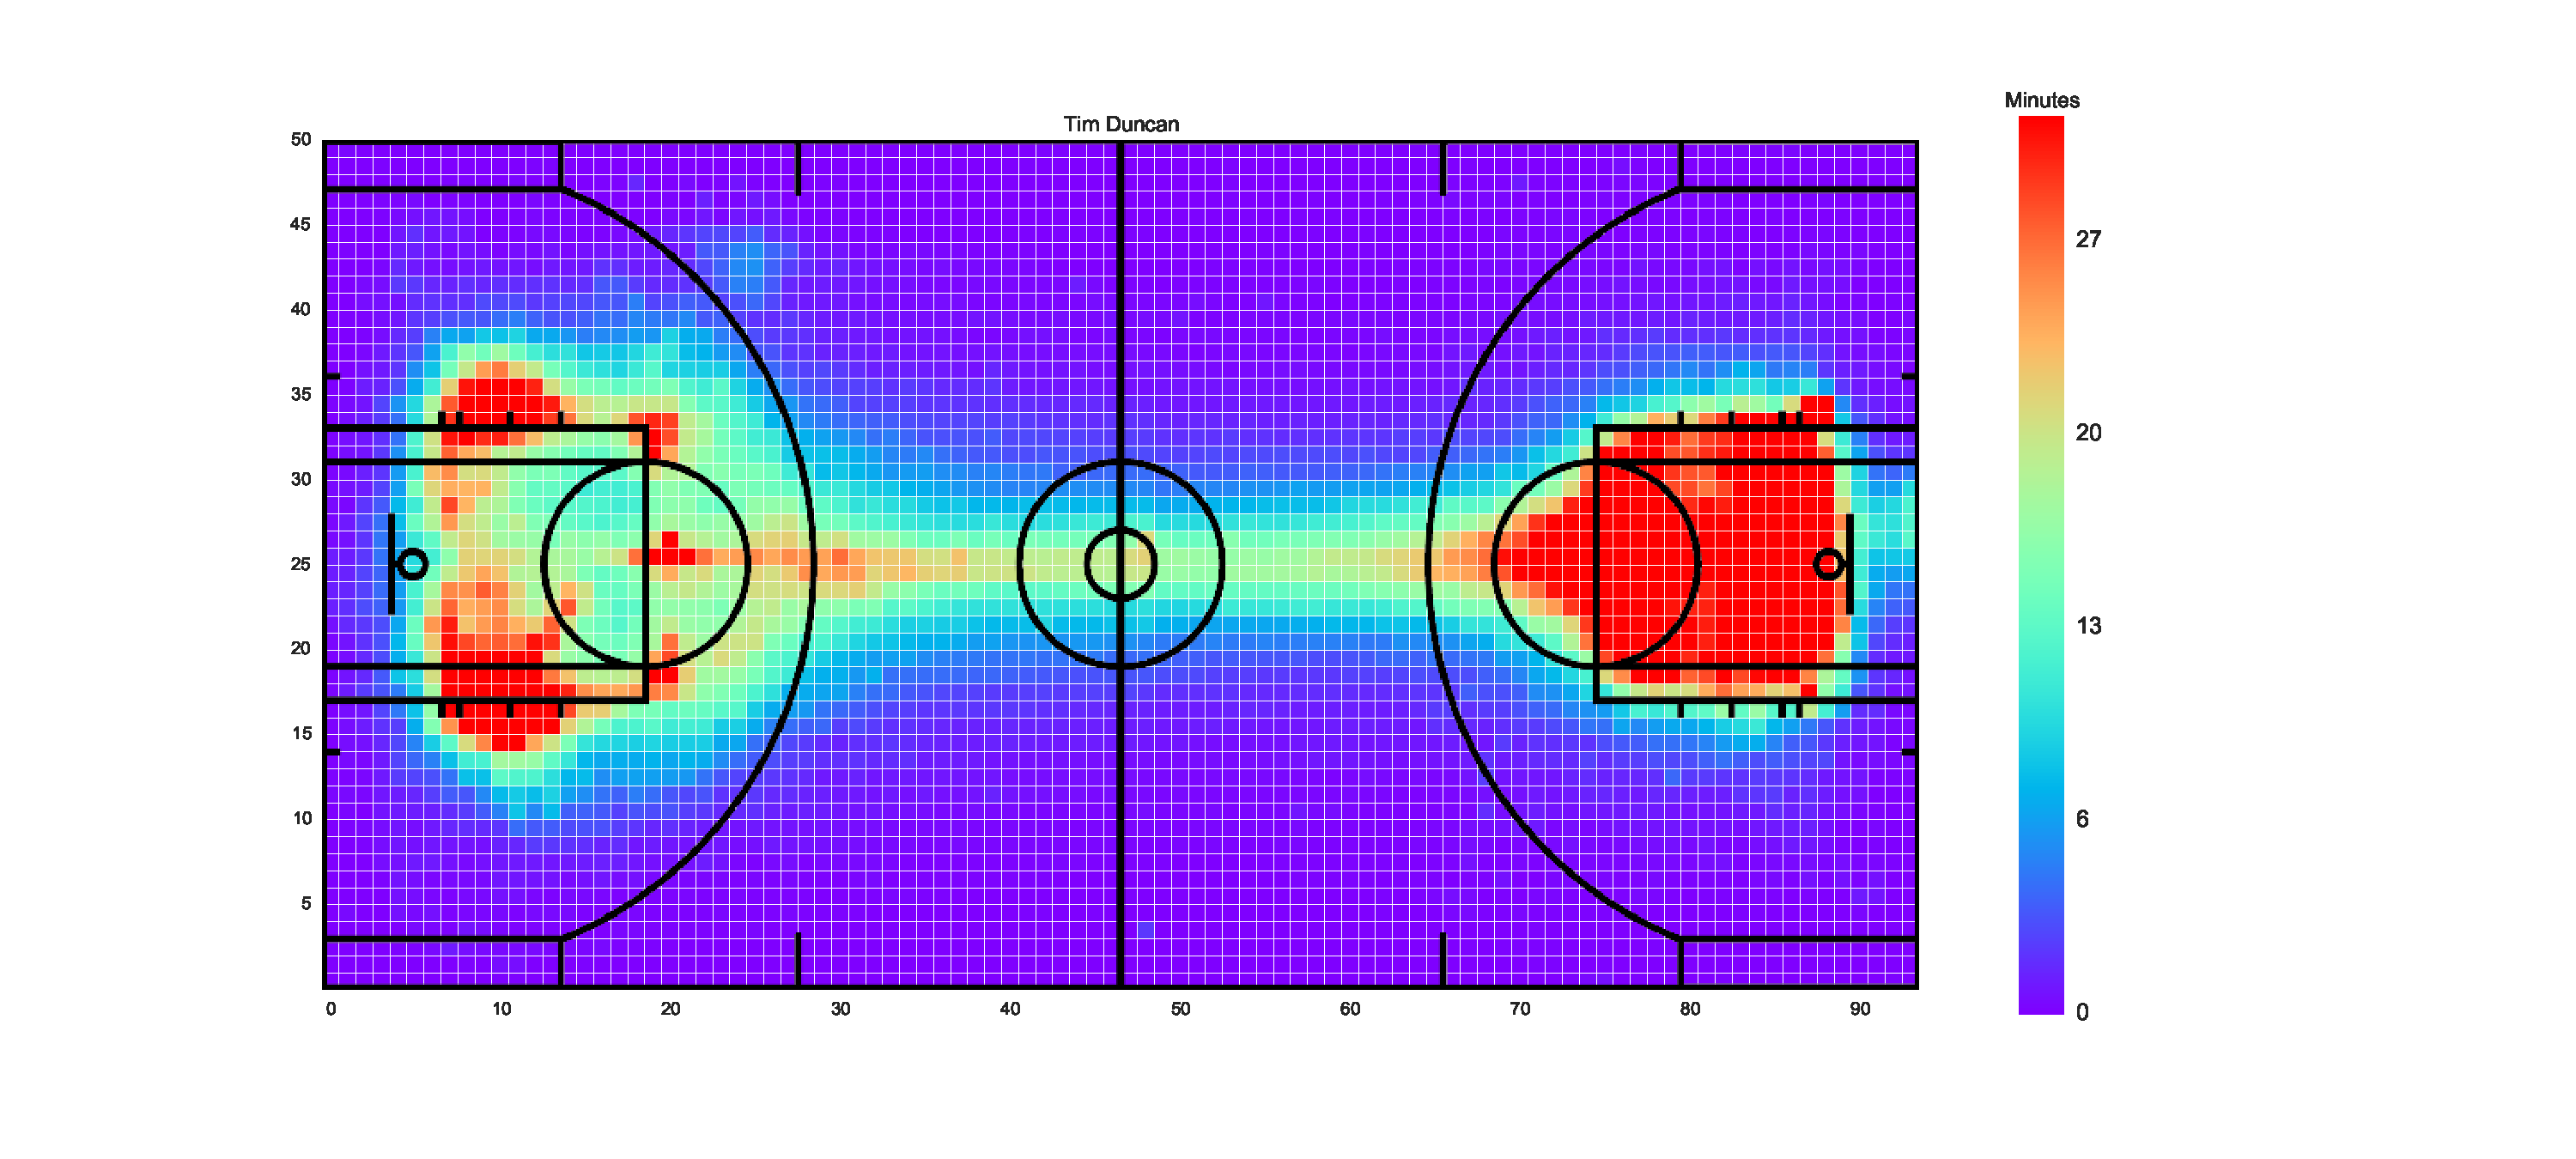
\includegraphics[scale=0.4]{Tim_Duncan_heat_rainbow.pdf}

From here, we can linearize the distribution, and input the vector into a clustering algorithm. 
\section{Demo - Data Processing}
The tracking data are big - a single game is 20-25 MB compressed, and contains approximately 1 million $moment$ rows, as well as game and player metadata. The first month of the 2015 season is 6 GB compressed. The data was collected with a MapReduce framework in mind. 

\noindent The code expects that the data are organized on the server like this:
\begin{footnotesize}
\begin{verbatim}
path_to_tracking_data/
    2015-10-31/
        scoreboard-20151031.json
        0021500033/
            game_0021500033-playbyplay.json.gz
            game_0021500033-play_001.json.gz
            game_0021500033-play_002.json.gz
            ...
            game_0021500033-play_459.json.gz
        0021500034/
            ...
        0021500035/
            ...
    2015-11-01/
        ...
\end{verbatim}
\end{footnotesize}

\subsection*{Local Implementation}

\noindent We see that there is a directory for each date, which contains a directory for each game on that date. Inside each game directory, there are 300 to 500 different JSON play files.

To process and run analysis code across all games of the tracking data, our processors follow a standard map/reduce pattern. First, we run an independent function, $process\_game()$, in each game directory (the map phase). Then, we can manipulate the results using a $process\_results()$ function (the reduce phase).

The local implementation is using python, and takes approximately 30 seconds per game





\subsection*{Hive Implementation}
The Hive implementation so far was done using a subset of the NBA season data, containing only 3 games. That yielded around 2.3 million rows for locations data (main table) and 78 rows with player data (aux table).\\
\\ The query used for the critical part of this project (which is aggregating the count of locations by player) took in average 73s. When we partitioned the table by player\_id it performed consistently faster, in average 63s (13\% improve).\\
\\ For the last week of the project, we are gonna use the entire data and try other partitions, pick the fastest and compare to the other implementations.\\
\\Below is the code used for the Hive part: \\

\begin{lstlisting}
/* Setting AWS keys to access data in S3 buckets */
SET fs.s3n.awsAccessKeyId = <secret key id>;
SET fs.s3n.awsSecretAccessKey = <secret access key>;

/* Setting parameters to properly partition data */
SET hive.exec.dynamic.partition=true;  
SET hive.exec.dynamic.partition.mode=nonstrict; 

CREATE EXTERNAL TABLE players (player_id STRING, team STRING, 
first_name STRING, last_name STRING, position STRING)
ROW FORMAT DELIMITED FIELDS TERMINATED BY ','
LOCATION 's3n://dcproject-public/players/';

CREATE EXTERNAL TABLE locations (row_number STRING, game_id STRING, 
unix_time STRING, quarter INT, team_id STRING, player_id STRING, 
game_clock FLOAT, shot_clock FLOAT, x FLOAT, y FLOAT, z FLOAT)
ROW FORMAT DELIMITED FIELDS TERMINATED BY ','
LOCATION 's3n://dcproject-public/locations/';

CREATE TABLE locations_part (game_id STRING, quarter INT, team_id 
STRING, game_clock FLOAT, shot_clock FLOAT, x FLOAT, y FLOAT, z FLOAT)
PARTITIONED BY (player_id STRING)
ROW FORMAT DELIMITED FIELDS TERMINATED BY ',';
LOCATION 's3n://dcproject-public/locations_part/';

INSERT OVERWRITE TABLE locations_part PARTITION (player_id)
SELECT game_id, quarter, team_id, game_clock, shot_clock, x, y, z, 
player_id FROM locations;

/* Main query to aggregate the whole thing (no partition): */
select concat(players.first_name,'_', players.last_name) name, l.x, 
l.y, l.cnt from (select player_id, x, y, count(*) cnt from (select 
player_id, round(x, 0) x, round(y, 0) y from locations where 
player_id <> -1) a group by player_id, x, y) l left join players 
on l.player_id = players.player_id order by name, x, y limit 20;

/* Main query to aggregate the whole thing (partition by player_id): */
select concat(players.first_name,'_', players.last_name) name, l.x, 
l.y, l.cnt from (select player_id, x, y, count(*) cnt from (select 
player_id, round(x, 0) x, round(y, 0) y from locations_part where 
player_id <> -1) a group by player_id, x, y) l left join players 
on l.player_id = players.player_id order by name, x, y limit 20;
\end{lstlisting}

And here is the sample results (first 20 rows) for the last queries (data partitioned by player\_id):\\

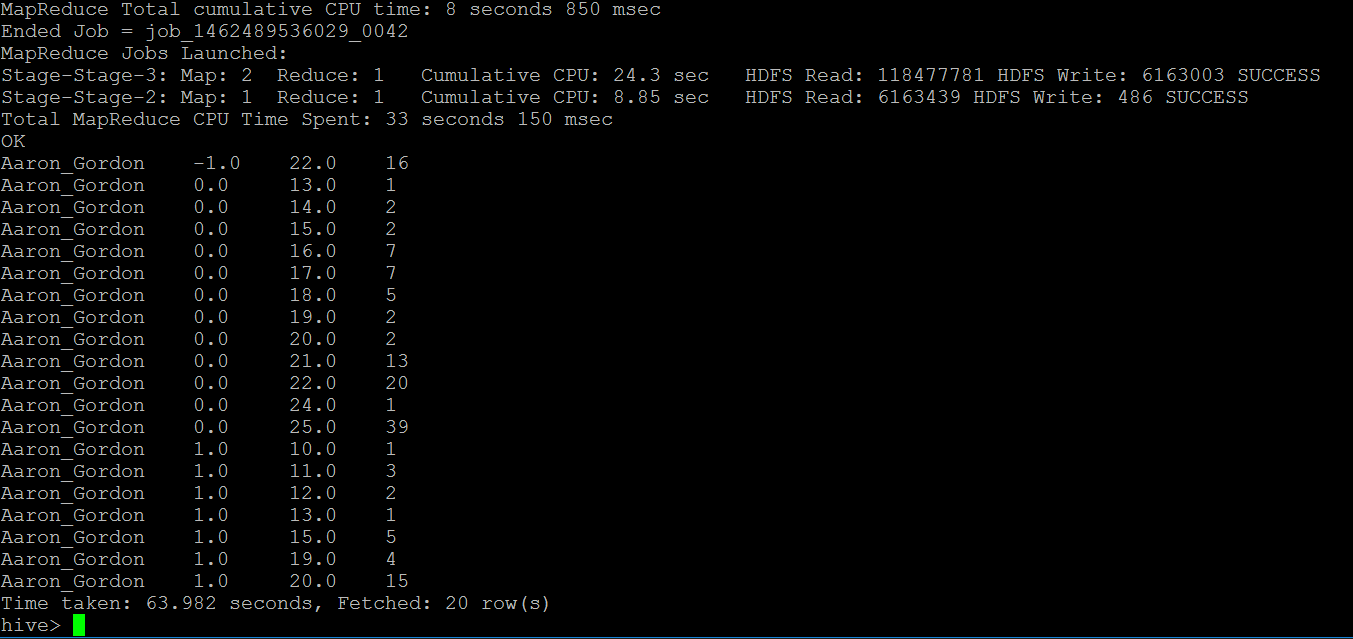
\includegraphics{results_hive_partition_player_id.PNG}

\end{document}